\documentclass[aps,pra,12pt,notitlepage,tightenlines]{revtex4-1}
%\usepackage[margin=2.5cm]{geometry}
\usepackage{amsmath,amssymb,textcomp,graphicx,url,bm,lipsum,hyperref,color,subcaption,afterpage,gensymb}

\newcommand\matr[1]{\bm{#1}}
\newcommand\barparen[1]{\overset{\textbf{\fontsize{5pt}{5pt}\selectfont(---)}}{#1}}

\graphicspath{{Images/}}

\newcommand{\nue}{$\nu_e$ }
\newcommand{\anue}{$\bar\nu_e$ }
\newcommand{\numu}{$\nu_\mu$ }
\newcommand{\anumu}{$\bar\nu_\mu$ }

\begin{document}

\title{Upgrading ND280 and an Overview of \nue and \anue Detection using an Anti-Neutrino Beam\vspace{0mm}}
\author{Wilf Shorrock\vspace{1mm}}
\affiliation{Imperial College London\vspace{-0.5mm}}
\date{\today}
\begin{abstract}
\linespread{0.97}
\vspace{1mm} In 2020, the T2K experiment is set to enter a new phase of data-taking with increased statistics. To make full use of the higher statistics and reduce systematic errors, upgrades to the near detector, ND280, have been proposed. In this report, after introducing the T2K experiment and describing the sub-detectors currently comprising ND280 and the structure of its software, the future upgrades will be outlined. The beam test performed at CERN for the prototype of the new Super-FGD detector that will be installed in the upgraded ND280 will also be described, along with preliminary results. An introduction to the detection of electron neutrinos at ND280 will also be included, which will lead in to the future work I will be carrying out for my PhD.
\end{abstract}

\maketitle

\newpage
\tableofcontents
\newpage

\vspace{-8mm}

\section{Introduction}
%In their 1956 paper announcing the discovery of the neutrino, Reines and Cowan stated:
%\begin{quotation}
% ``Each new discovery of natural science broadens our knowledge and deepens our understanding of the    physical universe; but at times these advances raise new and even more fundamental questions than those     which they answer~\cite{1956Natur.178..446R}.''
%\end{quotation}
%At the time, they were referring to the observation of beta decay and how it led to the proposal of the neutrino, but it is rather fitting that we can also apply this statement to the neutrino itself. Since the observation of atmospheric neutrino oscillations at Super-Kamiokande (SK) in the 1990s, a whole new area of research has opened up, and results from further experiments observing reactor neutrinos~\cite{PhysRevLett.108.171803, PhysRevLett.108.191802, PhysRevLett.108.131801} have shown that neutrinos oscillate between three flavour states via three mass eigenstates.

The imprint neutrinos leave on our world is almost unnoticeable due to their vanishingly small cross-sections with respect to everyday baryonic matter. Yet, the ethereal nature of the neutrino belies its importance in the Universe. Neutrinos have pervaded our world almost since the very beginning and they have affected the evolution of entire galactic systems. This is why physicists are persevering in their attempts to measure the properties of the almost undetectable neutrino, a study in which they have made noticeable progress over the past few decades. 

Since the neutrino was first discovered in 1956 by Reines and Cowan~\cite{1956Natur.178..446R}, the way in which it has been perceived by the scientific community has evolved significantly. After initially thinking all neutrinos were identical, we now know they come in three different flavours, each one conserving the number of a particular family of leptons in any interactions---albeit extremely rare interactions---they may take place in. The notion of neutrino mass is also a new concept, with the neutrino thought of as massless before it was discovered that neutrinos could oscillate in flavour by Super-Kamiokande (SK) in the 1990s~\cite{Fukuda1998}. This effect implies that neutrinos must have some mass, although to have been unmeasured thus far it must be extremely small.

Neutrino oscillation has become one of the more promising avenues towards Beyond Standard Model physics. It also helps to shed light on previously unexplained measurements, for example the lack of electron neutrinos originating from the Sun, solved by realising the electron neutrinos can oscillate and change flavour~\cite{PhysRevLett.89.011301}. 

There have been several experiments in the past measuring oscillation parameters using neutrinos produced in nuclear reactors, most notable Daya Bay, Double CHOOZ, Sudbury and RENO \cite{PhysRevLett.108.171803, PhysRevLett.108.131801, PhysRevLett.89.011301, PhysRevLett.108.191802}. There are still several reactor-based experiments today, as well as experiments using neutrino beams produced using particle accelerators. The goals of these experiments are to make more precise measurements of the oscillation parameters, and also try to ascertain whether charge parity (CP) is conserved or not in these oscillations.

Tokai to Kamioka (T2K) is a long-baseline experiment that studies accelerator neutrinos, which are the tertiary products of high energy protons striking a graphite target. Since it began taking data in 2010, T2K has made precision measurements of the oscillation parameters $\Delta m^2_{23}$ and $\sin^22\theta_{23}$ and one of the first measurements of the mixing angle $\theta_{13}$ (these parameters are explained in Sec.\ \ref{sec:osc})~\cite{PhysRevD.88.032002}. The latest analysis results were published in 2017~\cite{Abe:2017bay}. Over the next few years, the experiment will attempt to observe CP violation (CPV) in neutrino oscillations with at least a 3$\sigma$ statistical significance (if the CPV is maximal) and ascertain whether the mixing angle $\theta_{23}$ is maximal, as current measurements suggest. This new phase of the experiment is to be called T2K-II and will require several upgrades to the experiment's detectors.

This paper will provide an overview of the proposed upgrades to the T2K experiment's off-axis near detector, ND280, as well as a description of the beam test carried out with the prototype of one of the new sub-detectors, called the Super-FGD. The process of analysing the near detector's anti-neutrino data to ascertain the electron neutrino and electron anti-neutrino contamination of the beam will also be presented, with the goal of introducing the future work of the author. Firstly, though, the theory behind neutrino oscillation will be given, leading on to an overview of the T2K experiment and details on the current state of ND280 and it's software.

\section{Neutrino Oscillation Model}
\label{sec:osc}
For neutrino oscillations to exist, the neutrino flavour eigenstates, $(\nu_e, \nu_\mu, \nu_\tau)$, must be different to the neutrino mass eigenstates, $(\nu_1, \nu_2, \nu_3)$. In fact, it must be the case that the flavour eigenstates are coherent superpositions of the mass eigenstates. Hence, they can be equated using the equation
%Neutrino oscillations are well described by the Pontecorvo-Maki-Nakagawa-Sakata (PMNS) matrix, although this does not include the possibility of sterile neutrinos, the details of which are beyond the scope of this report. The PMNS matrix relates the three neutrino flavour eigenstates, $(\nu_e, \nu_\mu, \nu_\tau)$, to three mass eigenstates, $(\nu_1, \nu_2, \nu_3)$, through the equation

\begin{gather}
\label{eq:pmns}
 \begin{pmatrix}
 \nu_e \\
 \nu_\mu \\
 \nu_\tau 
 \end{pmatrix}
 =
 \begin{bmatrix}
 U_{e1} & U_{e2} & U_{e3} \\
 U_{\mu1} & U_{\mu2} & U_{\mu3} \\
 U_{\tau1} & U_{\tau2} & U_{\tau3}
 \end{bmatrix}
 \begin{pmatrix}
  \nu_1 \\
 \nu_2 \\
 \nu_3 
 \end{pmatrix}
 ,
\end{gather}
where the matrix enclosed by square brackets is the Pontecorvo-Maki-Nakagawa-Sakata (PMNS) matrix, $\matr{M}_\mathrm{PMNS}$. The matrix elements $U_{\alpha i}$ represent the mixing amplitudes of mass state $i$ contained within flavour state $\nu_\alpha$.

Eq.\ \eqref{eq:pmns} encapulates all the physics of neutrino oscillations. It implies that, following the weak decay $W \rightarrow l_\alpha\nu_\alpha$, where $\nu_\alpha$ is a neutrino flavour eigenstate and $l_\alpha$ is the corresponding charged lepton state with flavour $\alpha$, the neutrino will propagate as a mixture of the mass eigenstates, which interfere quantum mechanically in interactions. This allows the neutrino to behave later in time as if it had a different flavour, where the probability of this flavour is dependent on the distance the neutrino travelled~\cite{Kayser:2005cd}. 

$\matr{M}_\mathrm{PMNS}$ is a unitary matrix, so it can be parametrised using three real angles, $(\theta_{12}, \theta_{13}, \theta_{23})$, and a real phase, $\delta_\mathrm{CP}$, to give
\begin{gather}
 \matr{M}_\mathrm{PMNS} = 
 \begin{bmatrix}
 1 & 0 & 0 \\
 0 & C_{23} & S_{23} \\
 0 & -S_{23} & C_{23}
 \end{bmatrix}
 \begin{bmatrix}
 C_{13} & 0 & S_{13}e^{-i\delta_\mathrm{CP}} \\
 0 & 1 & 0 \\
 -S_{13}e^{i\delta_\mathrm{CP}} & 0 & C_{13}
 \end{bmatrix}
 \begin{bmatrix}
 C_{12} & S_{12} & 0 \\
 -S_{12} & C_{12} & 0 \\
 0 & 0 & 1
 \end{bmatrix}
 ,
\end{gather}
where $C_{ij} = \cos\theta_{ij}$ and $S_{ij} = \sin\theta_{ij}$. These mixing angles and phases are what oscillation experiments aim to measure, as they encapulate the physics of the phenomenon. A non-zero value of the $\delta_{CP}$ phase (given that $S_{13}\neq 0)$ would mean that neutrino oscillations are CP-violating. There may be two extra phase parameters required if neutrinos are Majorana particles (Majorana particles are their own anti-particles) but these have no effect on oscillation measurements~\cite{Kayser:2005cd}.

For a detatiled derivation of the neutrino oscillation probabilities, see Kayser~\cite{Kayser:2011jn}. Here, we will quote the end result only, which is the probability of a \mbox{(anti-)neutrino} with initial flavour $\alpha$ and energy $E_\nu$ propagating a distance $L$ and being detected with flavour $\beta$:
\begin{align}
\label{eq:p}
P\Big(\barparen{\nu_\alpha}\rightarrow\barparen{\nu_\beta}\Big) = \delta_{\alpha\beta}&-4\sum^3_{i<j}\Re[U_{\alpha i}U_{\beta i}^*U_{\alpha j}^*U_{\beta j}]\sin^2\bigg(\Delta m^2_{ij}\frac{L}{4E_\nu}\bigg) \notag \\
& \mp 2\sum^3_{i<j}\Im[U_{\alpha i}U_{\beta i}^*U_{\alpha j}^*U_{\beta j}]\sin\bigg(\Delta m^2_{ij}\frac{L}{2E_\nu}\bigg),
\end{align}
where $\Delta m^2_{ij} = m^2_i - m^2_j$ is the difference between the squared masses of mass eigenstates $i$ and $j$. In fact, $\Delta m^2_{ij}$ is another set of parameters that oscillation experiments attempt to measure, in lieu of the absolute masses of each neutrino flavour.

Eq.~(\ref{eq:p}) can only be applied to neutrinos travelling through a vacuum. For neutrino propagation through matter, see the report by Kayser~\cite{Kayser:2005cd}.

\section{T2K}
The T2K experiment spans 295~km from the east coast of the main Japanese island, Honshu, to the west coast. The size of the experiment is one of it's advantages, as it enables sampling of areas of the parameter space that shorter baseline experiments can't access. 

The neutrino beam of T2K is generated at the Japan Proton Accelerator Research Complex (J-PARC) in Tokai. The beam is directed towards the other end of the experiment in Kamioka, travelling in a straight line through the Earth's crust. In Tokai, the beam passes through two near detectors---INGRID and ND280---that are 280~m from the beam's origin. At Kamioka, the beam reaches the far detector, SK. An illustration of the experiment is shown in Fig.\ \ref{fig:t2k}.
\begin{figure}
 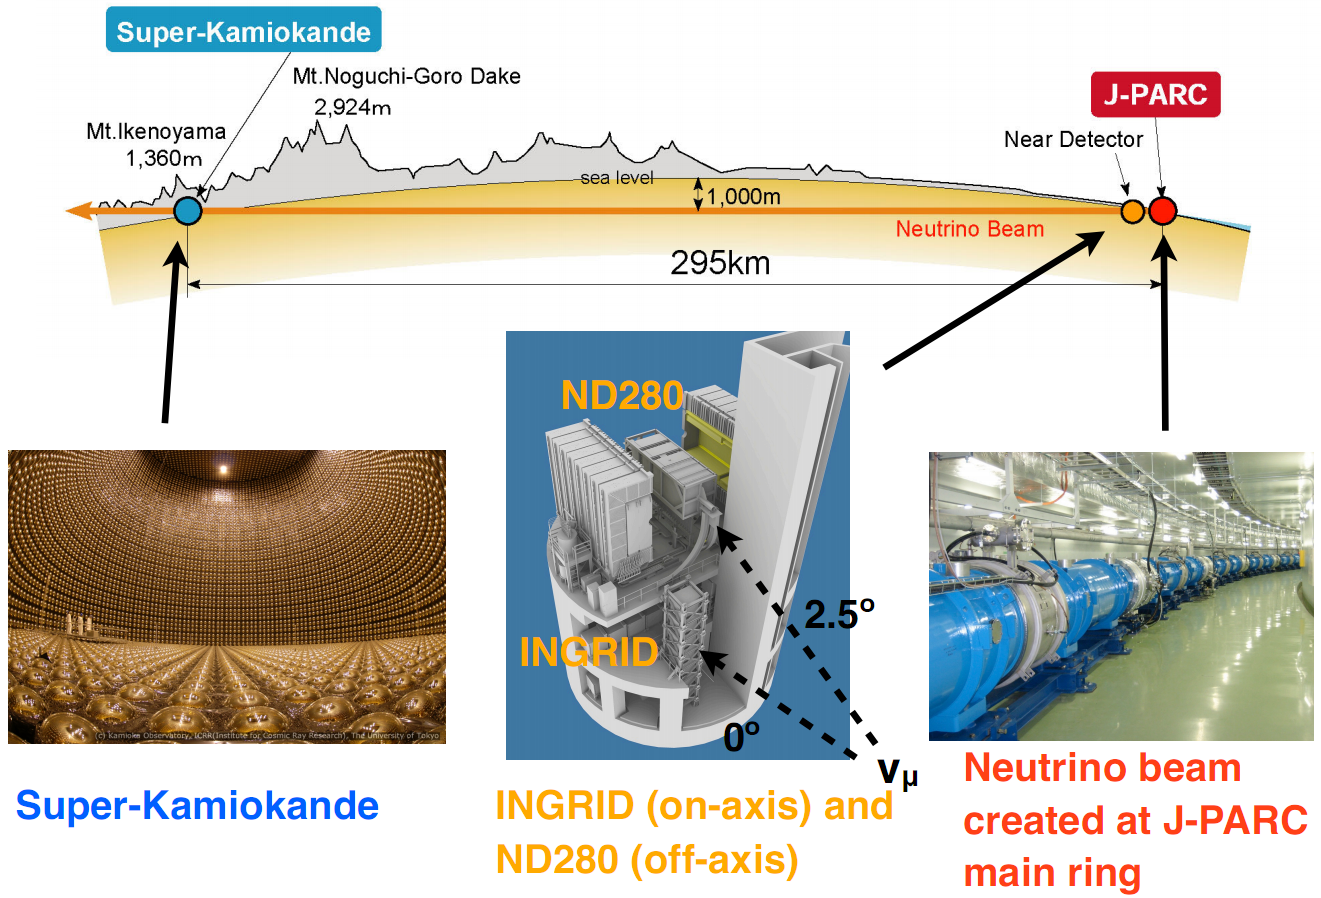
\includegraphics[scale=0.33]{T2K_detail}
 \caption{A diagram showing the path of the neutrino beam produced in the T2K experiment, along with illustrative photos/models of each major stage of the beam~\cite{Jamieson:2015rza}.}
 \label{fig:t2k}
\end{figure}

The INGRID detector lies on the axis of the neutrino beam, but ND280 and SK are 2.5\degree\ off-axis, which sets the peak of the neutrino flux at 600~MeV, the energy at which muon neutrino disappearance is most likely. Fig.\ \ref{fig:axis} 
\begin{figure}
 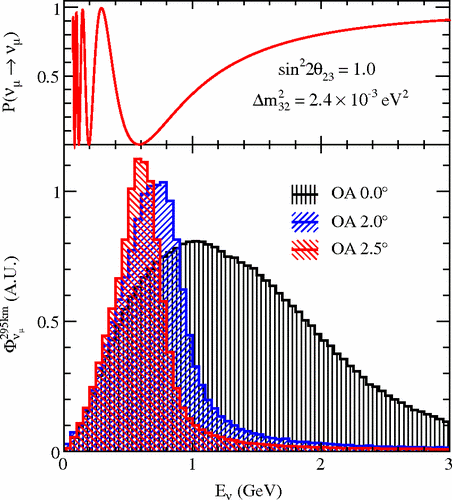
\includegraphics[scale=0.5]{axis.png}
 \caption{A plot (top) of the probability of muon neutrino survival as a function of energy, and a plot of the neutrino beam energy flux (bottom) for several off-axis angles.}
 \label{fig:axis}
\end{figure}
shows the flux of the neutrino beam as a function of neutrino energy at several different off-axis angles. Also shown is the probability of a muon neutrino keeping its muon flavour as a function of neutrino energy. It is clear that the peak flux for a 2.5\degree\ off-axis angle occurs at the same energy as one of the minimum points in the probability plot.

The content of the neutrino beam used in T2K can be switched between muon neutrinos (\numu) and anti-muon neutrinos (\anumu). The neutrinos are produced from the decay of muons, which are focused by electromagnetic horns. Reversing the current passed through the horns causes particles of opposite charge to be focused, hence one can focus muons or anti-muons depending on the current's direction. The mode in which muons are focused to give a \numu beam is the forward horn current (FHC) mode, and to focus anti-muons and create a \anumu beam the reverse horn current (RHC) mode is needed.

In the next section, we will give details on T2K's ND280 detector and its proposed upgrades for the next phase of data-taking. Information on the other T2K detectors and the beamline is given elsewhere~\cite{ABE2011106}.

\section{ND280: Current State}
ND280---so called because it is a Near Detector 280~m away from the neutrino beam's origin---gathers data on the neutrino beam to estimate the beam's flux, energy spectrum, and flavour content. This allows comparison with measurements at the far detector, leading to calculations of neutrino oscillation parameters by observing how the flavour content of the beam has changed as a function of energy. 

As well as monitoring the beam characteristics, ND280 also takes data for neutrino cross-section measurements, helping to provide a more accurate analysis of the oscillation data. 

The detector itself can be broken down into four main systems: a $\pi^0$ detector (P\O D), a tracker consisting of several fine grain detectors (FGDs) and time-projection chambers (TPCs), an electromagnetic calorimeter (ECal), and the side muon range detector (SMRD). The whole detector is subject to a 0.2~T magnetic field for particle identification (PID) and momentum determination. See Fig.\ \ref{fig:ND} for a visualisation of the ND280 detector and its sub-detectors.
\begin{figure}
 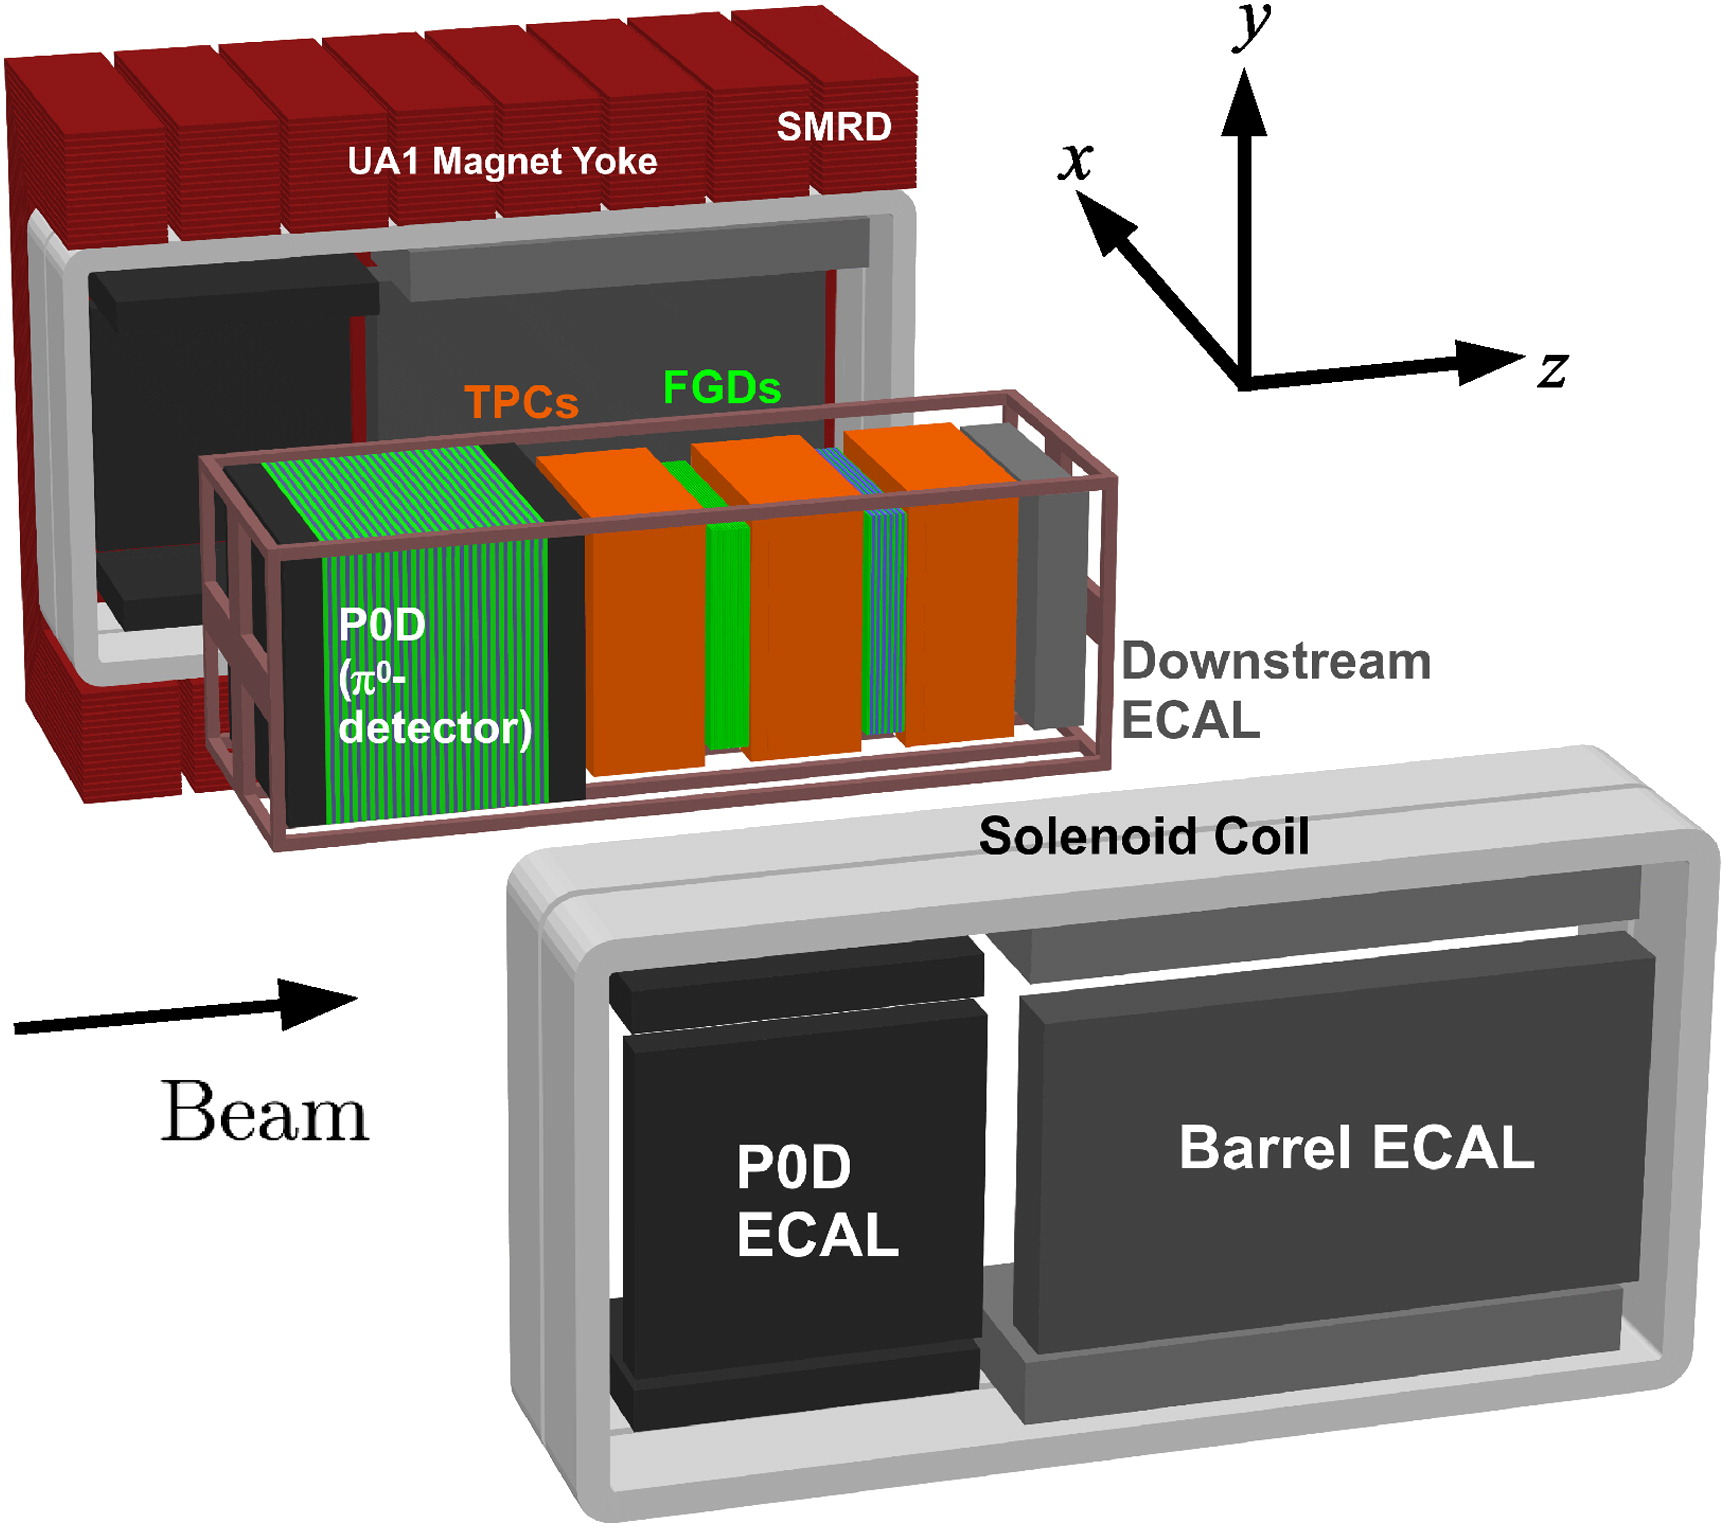
\includegraphics[scale=1]{ND280.png}
 \caption{Expanded view of the ND280 detector, showing the positions of each of the three main sub-systems and sub-detectors. The entire detector is encased in the UA1 magnet with a 0.2~T magnetic field~\cite{ABE2011106}.}
 \label{fig:ND}
\end{figure}

The sub-detectors of ND280 will now be described in more detail, apart from the SMRD, which can be read about in the literature~\cite{Aoki2013}. An introduction to the software used by ND280 will also be given.

\subsection{$\pi^0$ Detector (P\O D)}
T2K's far detector, SK, has difficulty discerning between electrons and pions. To reduce this systematic error, the P\O D sub-detector of ND280 is used to measure the cross-sections of neutrino interactions, specifically with water, where a neutral pion ($\pi^0$) appears in the final state. Using this cross-section data, the number of $\pi^0$s produced in SK can then be calculated and taken into account.

The central section of the P\O D consists of alternating layers of brass, plastic scintillator, and fillable water bags. The brass acts as a radiator and the water and target layers provide a target for neutrinos to interact with. The scintillator emits photons when a charged particle passes through it. This is exploited by using wavelength shifting (WLS) fibres to read off the light signal from a passing particle and using the data to reconstruct the particle's trajectory. 

The central target is preceded and followed by electromagnetic calorimeters comprised of alternating sheets of lead and scintillator. The ECals are used for rejecting particles entering the P\O D that originated from outside the detector and also to contain and measure electromagnetic showers. 

Cross-section values with respect to the water target can be deduced by taking measurements when the target bags in the central section are filled with water and comparing them to when they filled with air~\cite{ABE2011106, Assylbekov:2011sh}.

\subsection{Fine Grain Detectors (FGDs)}
The FGDs provide mass with which incoming neutrinos can interact and precision tracking to map out the interaction vertices. They consist of bars of plastic scintillator oriented perpendicular to the neutrino beam and stacked to form sheets. Two sheets are placed one after the other to form a module, with the bars of one layer being arranged vertically (along the $y$-axis) and the other layer horizontally (along the $x$-axis). The bars are read-off by WLS fibres, so the position of a charged particle incident on a module can be determined in two dimensions. Placing several modules in sequence then gives the trajectory of a particle through the detector

There are two FGDs in ND280. The downstream FGD also contains layers of water in between the scintillator layers. Comparing interaction rates between the two FGDs allows calculation of the cross-sections of neutrino interactions with carbon and water~\cite{ABE2011106, Amaudruz:2012agx}.

\subsection{Time Projection Chambers (TPCs)}
There are three TPCs in ND280, sandwiching the two FGDs. The bulk of each TPC consists of an argon-based gas. When charged particles pass through this gas, they ionise the gas molecules. The ionisation electrons drift away from a cathode and towards a readout plane. The location and arrival time of the electrons on this plane can be used to construct a 3D image of the particle's trajectory.

TPCs are ideal for identifying the number and trajectory of charged particles in the detector, although their relatively small mass makes it unlikley for a neutrino to interact with them, hence the need for FGDs. The information provided by TPCs allows selection of low-contamination interaction samples, as well as momentum measurements from curved tracks caused by the magnetic field present in the detector. Combining a particle's momentum along with the ionisation of the particle's track, one can identify the type of particle that made the track. Hence, when combined with the FGD data, the TPCs can be used to help estimate the neutrino flux as a function of energy and to determine the contamination in the muon neutrino beam by electron neutrinos~\cite{ABE2011106, Abgrall:2010hi}.

\subsection{Electronic Calorimeter (ECal)}
As well as the ECals either end of the P\O D, there are also ECals surrounding the entire detector. A ``barrel'' ECal surrounds the tracker around the $z$-axis, another ECal is situated downstream of the tracker, and a third encircles the P\O D. %These ECals are arranged to try and minimise the number of particles that leave the detector without passing through an ECal. 

The main uses of the ECals are to complement the inner detectors by measuring the energies of photons missed by the inner detectors, reject particles from interactions outside the detector, and help with particle identification.

Alternating layers of scintillator and lead absorber make up each ECal. The scintillator layers consist of several bars of plastic scintillator. These bars are oriented perpendicular to the scintillator bars of the adjacent layers for $x$--$y$ tracking, similar to the FGDs~\cite{ABE2011106, Allan:2013ofa}.

\subsection{ND280 Software}
The ND280 software is used for offline analysis of data collected by ND280, as well as Monte Carlo (MC) data generation and analysis. The basic framework of the code was built in 2004, with the underlying structure and data storage relying on ROOT~\cite{Brun1997}, simulation libraries from Geant4~\cite{Agostinelli2003}, a package management system provided by CMT (Configuration Management Tool) \cite{Arnault:2000vu} and the version control system used to store each version of the code is CVS (Concurrent Version Systems) \cite{Berliner2001}.

A decision was made early-on in the software's lifetime to split the structure of the software into different packages, resulting in about 60 software packages in total~\cite{ABE2011106}. This offers easy access to specific areas of code and makes editing the software simpler for developers. 

The flow-path of the different data types through the package structure is shown in Fig.\ \ref{fig:struct} (only the most relevant packages are shown). 
\begin{figure}
 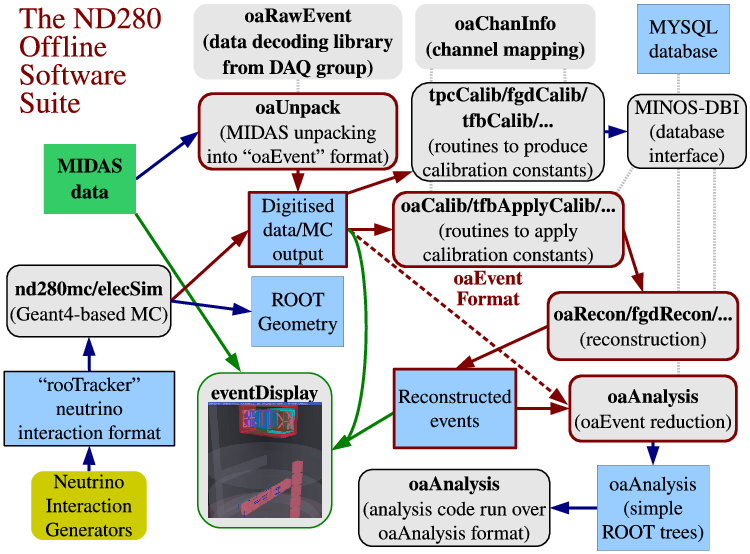
\includegraphics[scale=0.5]{struct.png}
 \caption{The flow of data through the package structure of the ND280 software. The flow is simplified and only shows the most relevant packages. Boxes with red coloured borders represent packages that process oaEvent data.~\cite{ABE2011106}}
 \label{fig:struct}
\end{figure}
The package oaEvent is important as it defines the format of the data passed through the software between the steps where raw MIDAS data (MIDAS is the format of data from the ND280 detector \cite{Ritt2001}) is passed to the software and the final step where oaAnalysis reduces the data to a user-friendly format. The oaUnpack and oaRawEvent packages handle the conversion of MIDAS data to oaEvent data. oaCalib then applies calibration constants to the data, whilst oaCalib's sub-packages use the data to produce calibration constants to store in MYSQL to be used by oaCalib. The data is then passed on to oaRecon, which uses the data to reconstruct the particle events that occurred in the detector, the results of which are analysed by oaAnalysis.

The exact same processes are applied to MC data, except that the data does not start in MIDAS format. The MC data is produced by passing information from the neutrino flux packages to the neutrino interaction generators NEUT~\cite{Hayato:2009zz} and GENIE~\cite{Andreopoulos2010}. These generators produce realistic distributions of child particles from neutrino interactions. The simulation is then taken over by nd280mc, which uses Geant4 to propagate the child particles and simulate the energy deposits left in the detector. elecSim then converts these energy deposits to simulated electrical readouts, as would be seen in the real detector and recorded in MIDAS format, except here it is written as oaEvent data.
 
\section{Hardware Upgrades}
Resulting from T2K's success in measuring oscillation parameters with improved precision, the experiment is set for a series of upgrades to further increase the measurement precision. In tandem with these improvements, ND280 must also be revamped to reduce statistical and systematic uncertainties in the neutrino appearance predictions. Here, we will go through the proposed upgrades, which are planned for construction over 2019--2020 to be installed in Japan by 2020~\cite{Blondel:2299599}.

\subsection{Scintillator Detector and Horizontal TPCs}
The proposed upgraded ND280 is shown in Fig.\ \ref{fig:up}.
\begin{figure}
 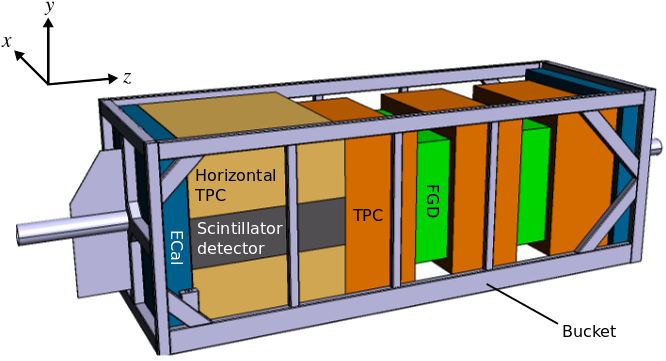
\includegraphics[scale=0.5]{upgrade2.png}
 \caption{The proposed upgrade of ND280. The new additions are the horizontal TPCs (light brown) and the scintillator detector (grey), which replace the P\O D. The ``bucket'' is a framework that supports the detectors. Not shown are the barrel ECals that will surround the detectors, similar to the original design. The neutrino beam propagates in the $z$ direction~\cite{Blondel:2299599}.}
 \label{fig:up}
\end{figure}
The downstream end of the detector will remain unchanged, with three TPCs separated by two FGDs. At the upstream end, however, the central P\O D module (not the ECal endcaps) will be replaced by a scintillator detector sandwiched between two horizontal TPCs. The scintillator detector will act as a target material, with the TPCs distributed around it giving nearly 4$\pi$ solid angle coverage. This  will address an issue with the old ND280 design: the tracking efficiency is biased towards low scattering angles. This is because, after a neutrino has interacted in an FGD, the resulting lepton is only seen in the downstream TPC if the scattering angle is less than $\sim$40\degree\ with respect to the beam direction. The TPC gives important information on the interaction, so most interaction samples exclude leptons with high scattering angles. This creates problems when comparing data with SK, which has a flat efficiency with respect to scattering angle.

The new scintillator detector will have a first-of-its-kind ``Super-FGD'' design that incorporates scintillator cubes rather than bars, which can be read out from three orthogonal directions by WLS fibres. The cubes' side length will be between 1--2~cm, with the larger lengths sacrificing granularity for a smaller number of cubes and readouts. The size of the cubes is comparable to the height and width of the scintillator bars used in the current design, but the bars only give readouts in two directions. The extra information provided by the cubes helps to reconstruct the paths of multiple particles. Fig.~\ref{fig:sfgd}
%\afterpage{
 \begin{figure}
  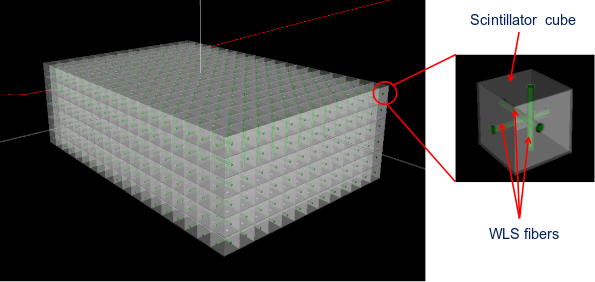
\includegraphics[scale=0.75]{SFGD.png}
  \caption{A rendering of the Super-FGD to be used in the upgraded ND280. The detector comprises many small plastic scintillator cubes that are read off in three orthogonal directions by wavelength shifting fibres. There are fewer cubes depicted here than there will be in the actual detector, to make the diagram clearer~\cite{Blondel:2299599}.}
  \label{fig:sfgd}
 \end{figure}
 %\clearpage
%}
shows an illustration of the Super-FGD design.

\subsection{Time of Flight Detectors}
Not shown in the diagram of the ND280 upgrade (Fig.\ \ref{fig:up}) are the new time-of-flight (TOF) detectors that are to be installed. These will be placed around the volume containing the scintillator detector and the horizontal TPCs. The TOF detectors will help identify whether a particle originated from inside or outside the detector, and will also aid with particle identification. The design of the TOF detectors is as yet undecided. There are two possible candidates, one based on wavelength shifting fibres and the other based on plastic scintillator bars. A prototype of the latter design is being constructed in 2018 and will be used in conjunction with the test-beam that will be run at the end of 2018. Prototypes of the horizontal TPC and the Super-FGD will also be used in the test-beam, the latter of which will be explained in more detail in the next section.

\section{Super-FGD Beam Test}
\label{sec:fgd}
The beam test for the Super-FGD prototype is scheduled for June 27th -- July 11th 2018, taking place at CERN.

The main goals of the beam test are:
\begin{itemize}
 \item Illuminate the detector with $\sim$1 GeV muons to collect data on the detector's properties like time resolution, position resolution, pulse height uniformity, alignment and more. This will also give an opportunity to calibrate the detector.
 \item Study the PID between electrons and gamma rays in the device and the two-track separation of electron-positron pairs by observing electron-pair production from gamma radiation.
 \item Measure energy loss of particles and study the effects of particles stopping in the detector.
 \item Collect samples of low energy protons from elastic scattering events with pions ($\pi^+ p \rightarrow \pi^+ p$).
 \item Observe high energy pion interactions that produce many particles to test multi-track separation.
\end{itemize}

At the time of submission for this report the beam test will be partially completed, making it difficult to relay results. I will be at CERN for the beam test and the weeks preceding it, so I will report on the set-up of the beam test, the prototype's design and the initial results, as well as describing my specific roles in the preparation and testing.

\subsection{The Super-FGD Prototype}
The prototype scintillator detector measures $24\times48\times8$ cm$^3$ and comprises 9216 extruded polystyrene mixed with p-terphenyl plastic scintillator cubes, each 1~cm long. There are a total of 1728 WLS fibres threaded through the cubes. On one end of each fibre is a connector, which attaches to another connector in which is housed a multiple photon pixel counter (MPPC) that sends a signal down a length of cable to the data acquisition (DAQ) system. Two photographs of the prototype are shown in Fig.\ \ref{fig:proto}.
 \begin{figure}
  \centering
  \begin{subfigure}{.5\textwidth}
   \centering
   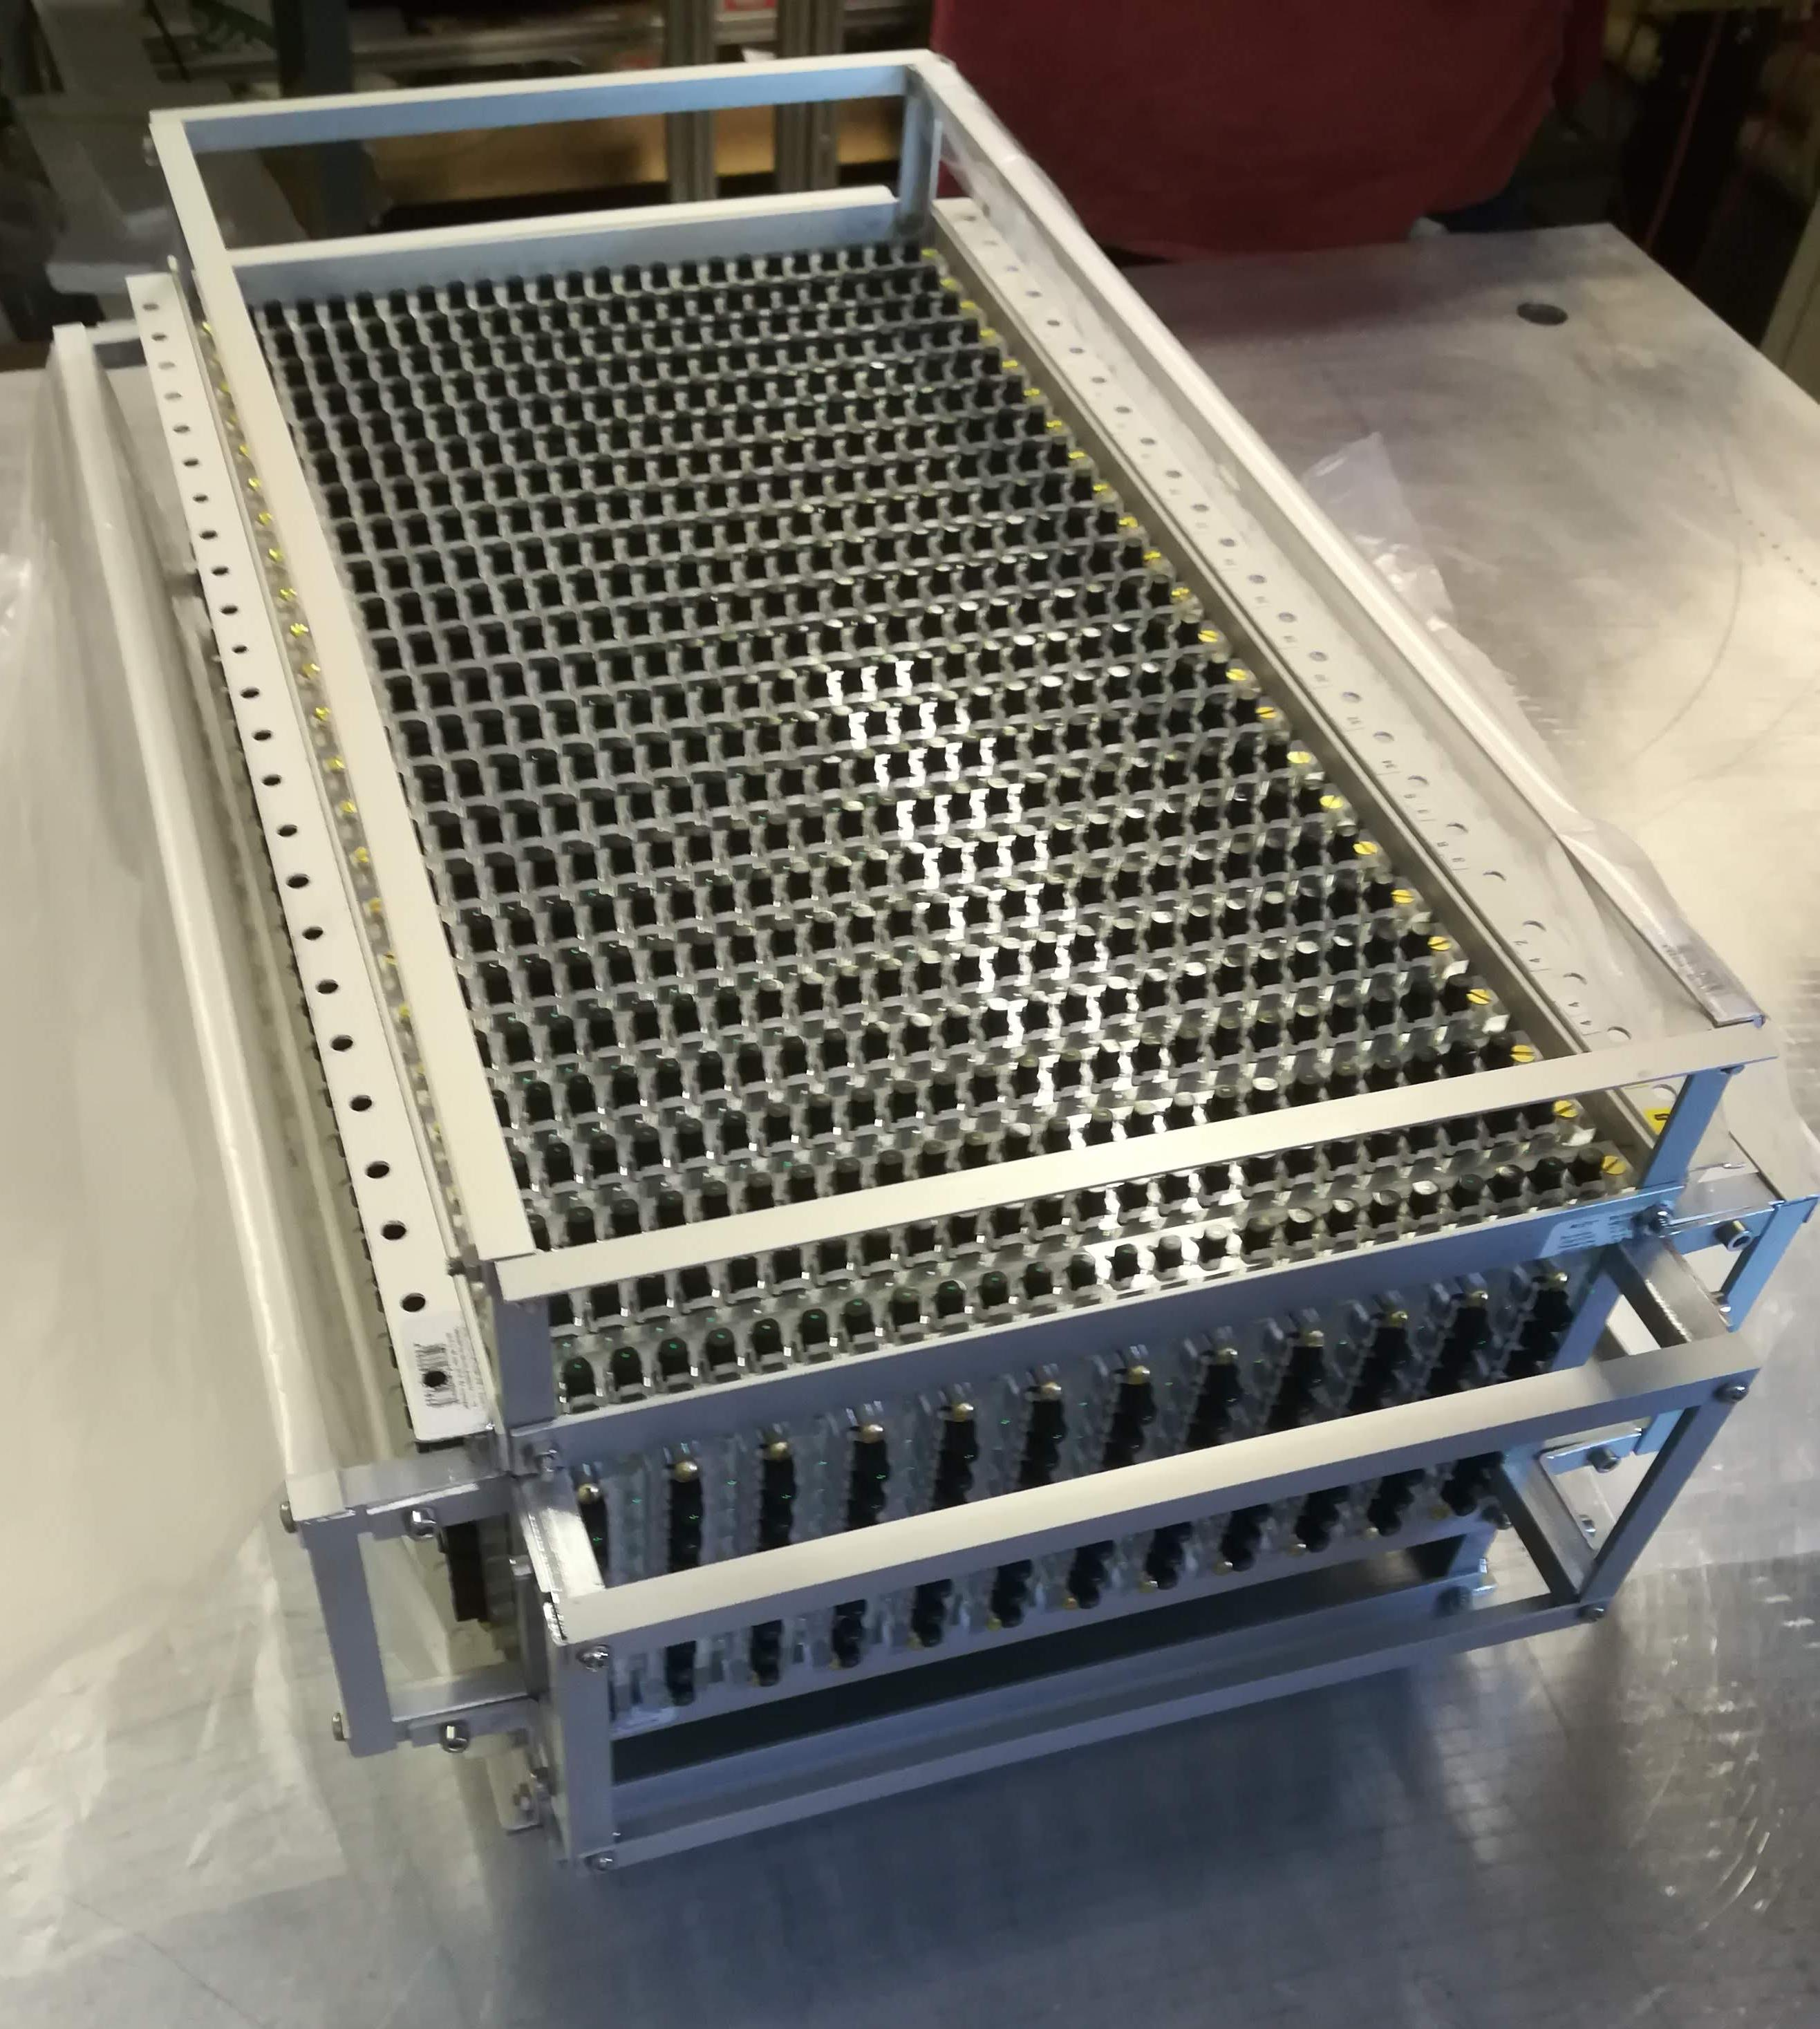
\includegraphics[width=.7\linewidth]{proto}
   \caption{•}
   \label{fig:protoa}
  \end{subfigure}%
  \begin{subfigure}{.5\textwidth}
   \centering
   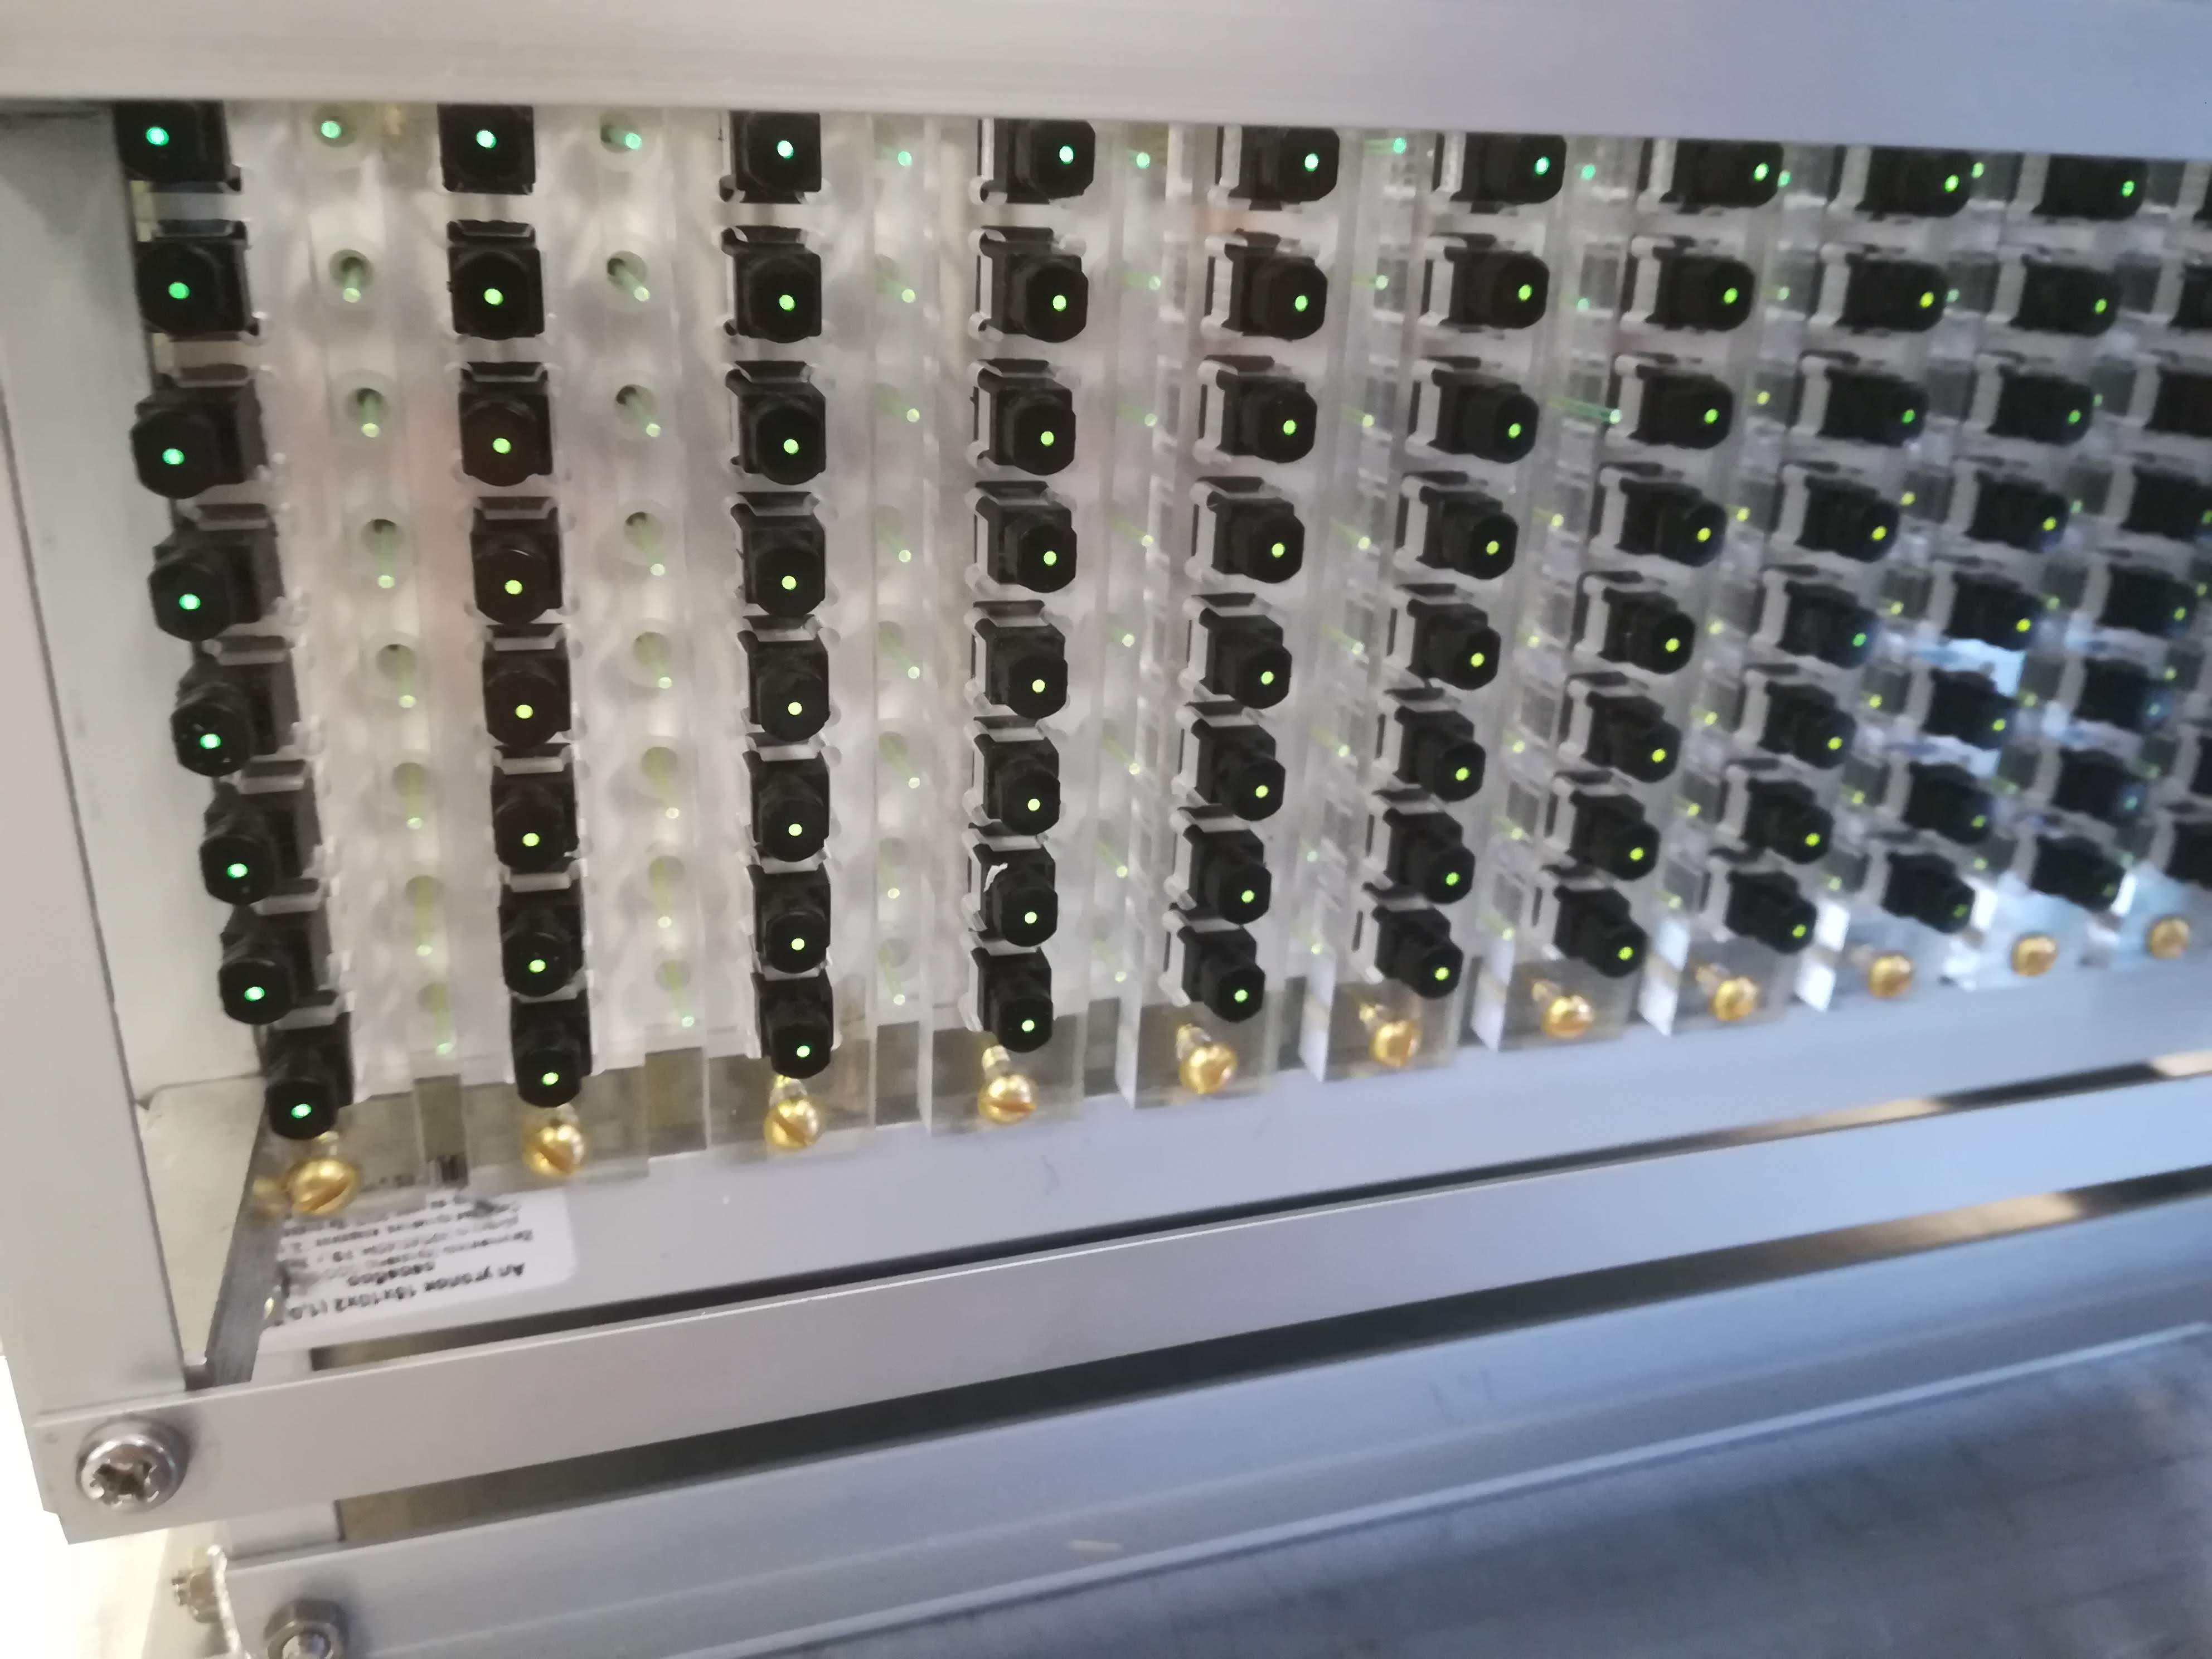
\includegraphics[width=.8\linewidth]{side}
   \caption{•}
   \label{fig:protob}
  \end{subfigure}
  \caption{Photographs of the Super-FGD prototype after being delivered to CERN. These were taken before the electronics were fitted for the beam test. (a) shows the whole detector, along with the frame it is housed in. (b) is a close-up of one of the detector's sides, giving a clear view of the scintillator cubes and the WLS fibres. The black connectors are where the readout electronics will be attached.}
  \label{fig:proto}
 \end{figure}
Fig.\ \ref{fig:protoa} shows the construct as a whole, housed in it's frame. Fig.\ \ref{fig:protob} displays a close-up of the side of the detector, giving a detailed view of the connectors at the ends of the WLS fibres, which will connect the detector to the DAQ system.

\subsection{The Beam Test Configuration} //TENSE??
The beam test is taking place in the East Area of the Proton Synchotron at CERN. Test-beam T9 is being used to fire $p, \ e^+, \ e^-, \ \pi^+, \ \pi^-, \ \mu^+$ and $\mu^-$ particles at the Super-FGD prototype with momenta ranging between 0.5--3~GeV (this is the expected momentum range for particles to be produced in the ND280 detector)~\cite{Durieu2001}. 

The prototype will be placed inside the MNP17 magnet, which is present for PID~\cite{Brooks2015}. The magnetic flux density will be set to 0.2~T, the same as the UA1 magnet of ND280. The readout electronics need to be placed outside the magnet field, hence long cables ($\sim$1.5~m long) are needed to connect the detector to the electronics. Fig.\ \ref{fig:plat}
\begin{figure}
 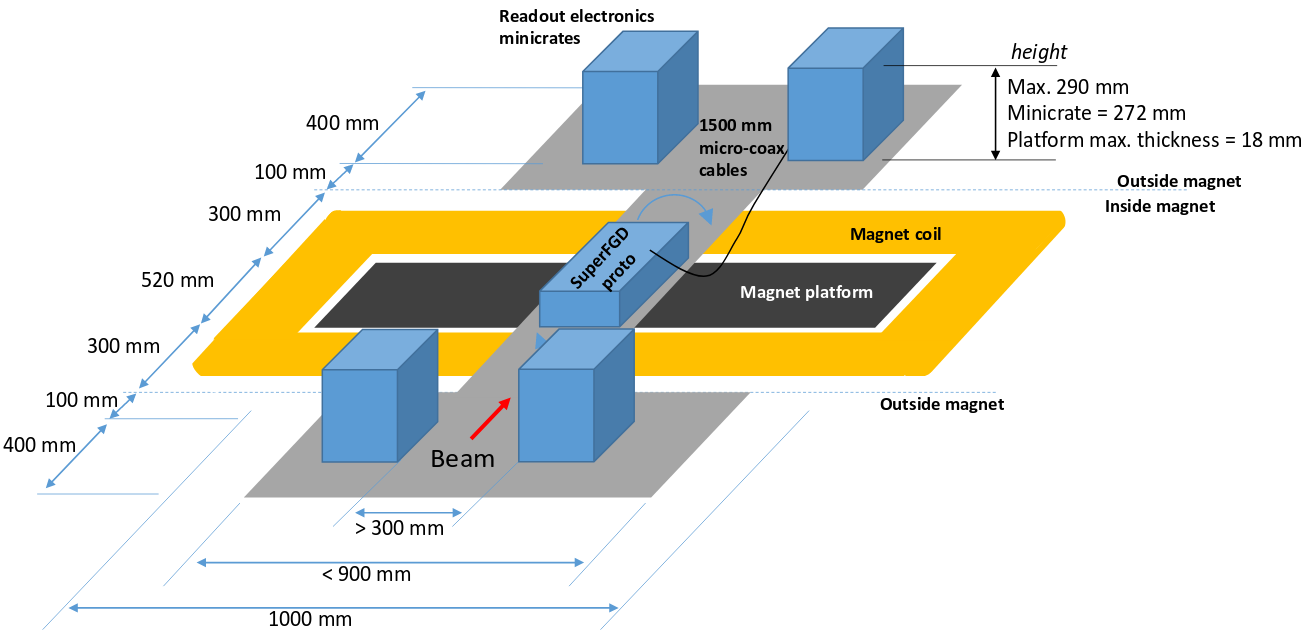
\includegraphics[scale=0.4]{platform2}
 \caption{A plan of the orientation of the prototype detector and its DAQ electronics with respect to the MNP17 magnet. Not shown is the upper platform of the magnet, which sits 290~mm above the lower platform. In order to access the prototype during the beam test, it will be placed on a mechanical platform that can slide out of the magnet. The platform will also rotate about the horizontal axis parallel to the beam and the vertical axis to allow different orientations of the prototype with respect to the beam~\cite{Cadoux2018}.}
 \label{fig:plat}
\end{figure}
shows how the detector is oriented with respect to the magnet, as well as the readout electronics, which are kept in metal boxes called ``minicrates''. The prototype is kept on a rotating platform so the detector's response to particles incoming at several angles can be tested.

The DAQ system in the minicrates is the same one that will be used for the Baby MIND detector~\cite{Antonova2017}. This will be used concurrently with another DAQ system using a WaveCatcher digitiser~\cite{CAEN}. This system will be connected to several hodoscopes and Cherenkov detectors, which will act as a trigger system and give PID. Baby MIND has it's own trigger system, so it's results will be compared with those of the WaveCatcher system, as a means of corroboration.

The layout of the detectors used in the trigger system is shown in Fig.\ \ref{fig:daq}.
\begin{figure}
 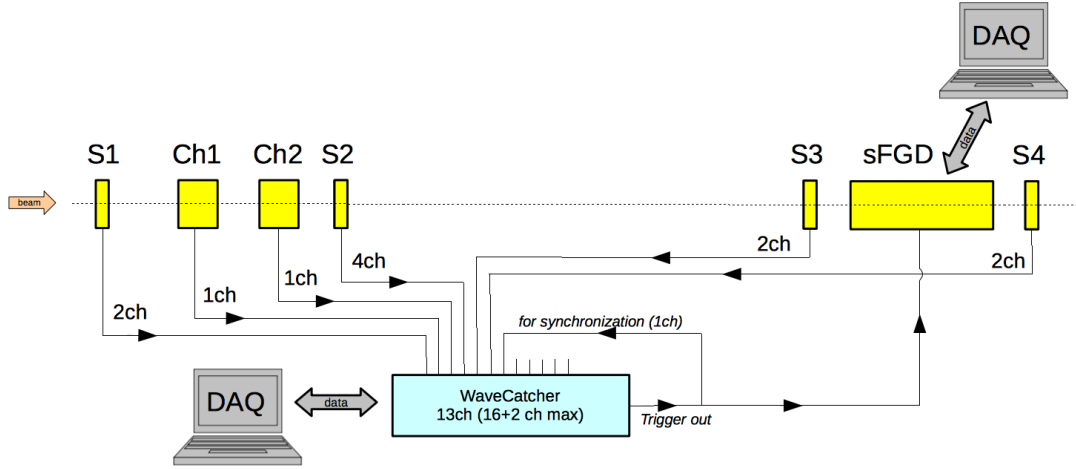
\includegraphics[scale=0.55]{daq}
 \caption{A schematic of the layout and DAQ for the beam test. The yellow boxes labelled S are beam scintillator counters and the ones labelled Ch are Cherenkov detectors. These are used in the trigger system for the Super-FGD prototype, labelled sFGD in the diagram. PID can be performed with the detectors in the triggering system by using time-of-flight and Cherenkov signals. There are two independent DAQ systems, one based on the WaveCatcher and the other Baby MIND, which is self-triggering. Also shown are the number of channels (ch) from each trigger component~\cite{Korzenev2018}.}
 \label{fig:daq}
\end{figure}
There are four hodoscopes in total, along with two Cherenkov detectors. By monitoring these detectors the trigger can be activated when a signal is produced in each one within a certain time window. Time of flight information can also be used to distinguish protons from other, lighter, particles. The Cherenkov detectors help with PID by distinguishing electrons from muons and pions. In the 0.5--3 GeV momentum range only electrons produce Cherenkov light in these detectors, making it easy to identify them.
%\subsection{Assembling the Prototype}

\subsection{Initial Beam Test Results}
//AWAITING RESULTS

\section{Software Changes}
There have been few changes to ND280's software structure since it was conceived 14 years ago, despite many new and upgraded software tools being introduced by developers. The proposal of an upgrade to ND280's hardware has sparked discussions of updates to the software, none of which will include a major overhaul of the framework, but will help streamline the code for the modern day developer. In this section, we will outline the changes that have been proposed following discussions from the ND280 software group, some of which are still subject to certain conditions and may change later on.

\subsection{Version Control}
CVS has been the version control system (VCS) of ND280 since it was first made. Back then, there were few alternatives and CVS seemed most suited to the task. More recently, however, advances have been made in the world of VCSs, with the introduction and popularisation of distributed systems. CVS is a centralised VCS. The difference between these two is that centralised VCSs require a master repository to which developers commit changes, but distributed VCSs allow developers to ``clone'' the software and all its metadata to a repository on their own hard drive. There are several advantages of distributed VCSs, including the ability to commit several changes at once, not requiring all developers of the project to see all the changes you make and not requiring an internet connection for actions other than pulling and pushing data to other repositories. //REWORD.

Given these advantages and many others, the ND280 software will be moved to a Git-based repository. It is most likely, though, that a frozen version of the latest software version at the time of migration will be kept on CMT, as means of a back-up. It's also possible that people can still commit changes to the CVS version after the migration, which will then be ported to the Git version, though this is still undecided.

There is also the question of which Git service to use. The choice is between GitHub, a popular VCS run on a //**commercial** server, which would require a paid subscription to keep the code stored there to be kept private. Alternatively, there is GitLab, a service specifically made with scientific experiments in mind, which requires a private server to be hosted. With this VCS the software will not be viewable by anyone, and specific levels of access can be given to individuals. There is also the benefit of built in continuous integration, a feature that makes the process of editing and committing code that much faster.

Following discussions in the software group, it has been decided that the ND280 software will be moved to GitLab rather than GitHub. GitLab offers several features that will be useful for scientific code development. There is also the recent news that GitHub has been purchased by Microsoft, so the future of GitHub and how it will operate is somewhat uncertain, making GitLab a safer and more reliable option. The University of Warsaw, Poland, has offered to host the private servers required to store the software on GitLab.

\subsection{Package Names}

COMET, another J-PARC experiment, which is searching for neutrino-less muon to electron decay, based it's software structure on that of ND280's~\cite{Wu2017}. In the process of editing the software for their specific use, they updated the package names to make them more consistent and clear. The imminent upgrade could be a good opportunity for ND280's software to follow suit, as there are some arguably confusing names and labelling rules.

A good example of COMET's updated package names is the renaming of the package elecSim to SimDetectorResponse. A developer new to the project would find it hard to discern the role of elecSim in the software (which is to simulate the electronics response of the detector), whereas SimDetectorResponse could not be much clearer. The example also highlights COMET's convention to add a prefix to each package name---such as ``Sim'' or in other cases ``Recon'', ``Calib'' and so on---that highlights where the package will be used in the data flow, i.e. in the simulation, the reconstruction, the calibration or something else. ND280 does this to an extent, but not as consistently, and a suffix is usually used rather than a prefix. 

Some other changes made by COMET were the use of capital letters. In ND280, most package names begin with lower-case lettering, but COMET have made each package begin with an upper-case letter (except packages with the ``oa'' prefix). This is a very basic change but one that arguably makes the names neater and easier to pick out in lists. A change was also made to the lettering of acronyms. For example, the package name ``fgdCalib'' in ND280 was changed to ``CalibFGD''. Again, this is a minor change but it makes the name much clearer and avoids confusion between acronyms and words.

From discussions by the ND280 software group, it seems likely that, when the software is migrated to a new VCS, the package names will be updated in a similar manner to the changes made by COMET, although the decision is not yet concrete.

\subsection{CMake and CMT}
The final applications of a software package need to be built after the software is edited or downloaded for the first time. From a developer's standpoint the performance of the build-tool is critical as they will have to build the software many times. A consumer of the software should only need to build the software applications once, so they are more concerned with the ease-of-use of the build tool. The creation and hierarchy properties of ND280's packages have so far been managed by CMT. Many other high energy physics experiments have used CMT with their software, but recently they have been switching to CMake~\cite{CMake}. One notable example is LHCb, who, until recently, maintained and used CMT before moving to CMake~\cite{Clemencic2012}.

CMake has an advantage over CMT through it's optimised code. This is especially useful on projects with a large number of packages, such as ND280, where CMT can perform significantly slower than CMake. One caveat, however, is the absence of some features that were present in CMT. The inheritance of link and compile flags, for example, is included in CMT. This is the process where, if one library (library1) is linked against another (library2), the paths to header files for library2 are included in the compile commands for library1, and all the libraries that were linked to library2 will be included in the link command to library1. In CMake, only the link command feature is included, and not the inherited paths for compile commands. This problem is surmountable because of the CMake language, which allows the construction of custom functions, including the implementation of compile flags. 

Overall, the advantages in performance most likely outweigh the work that would be required to include the missing features in CMake. Yet, there is currently still some debate as to whether ND280 should switch to CMake. It has clear advantages over CMT, but, on top of the extra effort of the implementation of features already included in CMT, many of the developers are unfamiliar with CMake, prompting the question of whether the move is worth the effort of learning the language of CMake. Currently, a few developers are attempting to build the ND280 software with CMake, and the results of their efforts will influence the decision of whether to stick with CMT or migrate to CMake.

\subsection{Mix-in Classes}
The software of ND280 currently uses ROOT5, but the latest version is ROOT6. It has been decided to update the software to integrate ROOT6, but in doing so a few things must be changed. The implementation of mix-in classes is the most notable issue. Mix-in classes are used in multiple inheritance, where the properties of several classes can be inherited. However, this is not implemented in ROOT6. The problem can be solved by replacing the implementation of the mix-in classes with C macros, but one would also need to alter the user code that accesses the mix-in classes.

To gauge how big of a job this would be, I performed a survey on the software to count the number of times mix-in classes are used (they can be identified by the ``TM'' prefix and ``State'' suffix in their name). The survey also identified the software packages and files each reference to the mix-in class was made in, but here I will only quote the final count of mix-in classes: five classes inherited a mix-in class and the mix-in classes are directly used in the code 50 times. This is relatively infrequent so the transition to ROOT6 shouldn't be significantly delayed by the reimplementation of these classes.

\section{\mbox{(Anti-)Electron} Neutrino Detection at ND280}
I am currently assisting with the production 7 analysis of anti-neutrino beam data from ND280 for \nue and \anue charged current interactions producing no pions ($\nu_e$/\anue CC-0 $\pi$ for short). Some electron neutrino contamination is expected in the muon neutrino beam produced at J-PARC, hence it is imperative to try and measure this at ND280 to reduce systematic errors when finding the number of muon neutrinos converted to electron neutrinos at SK.

The reference to ``production 7'' for the analysis refers to the build of the NEUT software used to generate MC data. The program is continually being improved with updated cross-sections and interaction models, so data is often re-analysed as part of a new production.

As I have only been on this project a few weeks, there are no results to show yet. Therefore, in this section I will introduce the reader to the cuts performed on ND280 anti-neutrino data for the production 6 analysis to isolate the \nue and \anue interactions. I will then go on to outline the rest of the analysis in the penultimate section on my future work for my PhD.

\subsection{Selection Cuts}
The selection of \nue and \anue interactions in ND280 is no easy task. There are several difficulties, such as the relatively small number of electrons produced in the interactions. Also, extremely accurate PID is needed to distinguish the electrons from other particles in the detector such as pions and protons. Not only this, there will be a large number of background electrons present from interaction of other particles, such as pions, which need to be rejected in the analysis. 

For PID and rejection of background electrons, a number of cuts are applied to the data. For the production 6 analysis, there were 12 cuts in total. I will give a concise list of them now.


\subsection{Production 6 Analysis}

\section{Future Work}
I will now outline how I will progress with my PhD by building upon my initial work and taking advantage of potential research opportunities in the future. It may be the case that the plan will not turn out to be entirely accurate, as other projects may unexpectedly present themselves or some of the proposed projects may fall through or be delayed, but I have attempted to include everything I can think of that I can complete during my PhD.

Following on from my work on the ND280 software, where I helped look at the different options for the software’s version control---its package naming, build methods, and the implementation of ROOT6---I plan to help with the transition of the software from the CVS repositories to GitLab. This will include implementing validation tests that check any uploaded code to ensure the software still runs correctly. I'm in a good position to carry out this work as I have access to the COMET repositories on GitLab and I am in contact with several COMET collaborators (COMET is another particle physics experiment with involvement from ICL) that can give advice on how they transitioned to GitLab.

Once the code is transitioned it will also need to be maintained. It is still to be decided whether a CVS build will be kept frozen or developed alongside the GitLab repositories, in which case it could be my duty to transfer data added to the CVS version to GitLab. Any other issues that arise such as updating package names could also be assigned to me.

Currently, the ND280 software is built using CMT, which creates the many packages that comprise the software. It has been decided that we will move on to using CMake instead of CMT, due to its flexibility and efficiency. It is still to be determined whether this transition will happen during the migration to GitLab or after. In either case I will be able to help implement the CMake build. I have some experience of the CMake language after studying the COMET implementation of their CMake build.

I am becoming familiar with the new Super-FGD detector to be installed for the ND280 upgrade in ∼2 years. I assisted with the beam test of the prototype at CERN, as outlined in section \ref{sec:fgd}. This could lead on to me helping with the analysis of the data from the beam test. From there I may also become involved with the actual Super-FGD and help to get it ready for installation at ND280.

I will also progress with my work on the production 7 analysis of electron neutrinos and anti-electron neutrinos at ND280 for the anti-neutrino beam data. I have read up on the production 6 analysis and am now in the process of reproducing their selection plots. My future work will move on to using the new production 7 Monte Carlo data in my analysis and extracting the electron neutrino and anti-electron neutrino composition of the beam and the detector systematic errors by performing fits on the data after selection cuts. I will also validate the results of the fits using Monte Carlo data.

Another potential project for me is the chance to perform an oscillation analysis using the latest data from T2K. This could form quite a large portion of the work I will include in my thesis, so it is important I become more familiar with the techniques and knowledge required for such an analyses.

%\section{Summary}

\bibliographystyle{mystyle}
\bibliography{bibliography.bib}

\end{document}
